\documentclass[final,a4paper,oneside,12pt]{article}
\setlength{\parindent}{0in}
 \usepackage{verbatim}
\usepackage{amsfonts}
\usepackage{amsmath}
\usepackage{color}
\usepackage{amssymb}
\usepackage[pdftex]{graphicx}
\begin{comment}
\usepackage[OT2,T1]{fontenc}
\DeclareSymbolFont{cyrletters}{OT2}{wncyr}{m}{n}
\DeclareMathSymbol{\Sha}{\mathalpha}{cyrletters}{"58}
\end{comment}
\usepackage{geometry}
%% Alex's thing
\setlength{\parskip}{0pt}
\setlength{\parsep}{0pt}
\setlength{\headsep}{0pt}
\setlength{\topskip}{0pt}
\setlength{\topmargin}{0pt}
\setlength{\topsep}{0pt}
\setlength{\partopsep}{0pt}
\linespread{1}

\geometry{
  body={7in, 10in},
  left=0.6in,
  top=0.5in
}

\setlength\parindent{0em}

\usepackage[compact]{titlesec}
\titlespacing{\section}{0pt}{*1}{*1}
\titlespacing{\subsection}{1pt}{*0.8}{*0.8}
\titlespacing{\subsubsection}{0pt}{*0}{*0}

\usepackage{amsfonts}
\usepackage{amsmath}
\usepackage{amssymb}
\usepackage[pdftex]{graphicx}
\usepackage{fullpage}
%%%
\begin{document}

\centerline{\Large \bf{RISE 2011 Report}}
\bigskip
\centerline{James McMurray - Physics student from the University Of Exeter, England}
\bigskip


\emph{I agree that my report and accompanying pictures may be used by the DAAD in printed materials, presentations, and on websites in order to inform funding organisations, sponsors, and students about the RISE programs (RISE, RISE pro and RISE worldwide).}\\

When I was first accepted on to the RISE programme, I was worried that the language barrier would be a great problem, and that I would struggle to find accommodation in time. Fortunately neither of these worries proved true, mostly due to the great hospitality shown by those I met. My internship was for 12 weeks at the Universit\"{a}t Konstanz in Konstanz near the border of Switzerland. I worked with the photovoltaics department, initially preparing Silicon samples and taking measurements and later writing software for data analysis.\\

Prior to leaving England, I emailed my PhD student supervisor and we discussed accommodation, eventually he found one of his friends who had needed someone to sublet with him as his flatmate was working abroad. However, because the other flatmate didn't leave until July, my PhD supervisor let me stay in his apartment for the last week of June when I first arrived in Konstanz. I also went sailing on the Bodensee with him and some of his friends. These are just some examples of the great hospitality I was shown.\\

%Herrenchiemsee image
\begin{center}
\begin{figure}[htp]
\centering
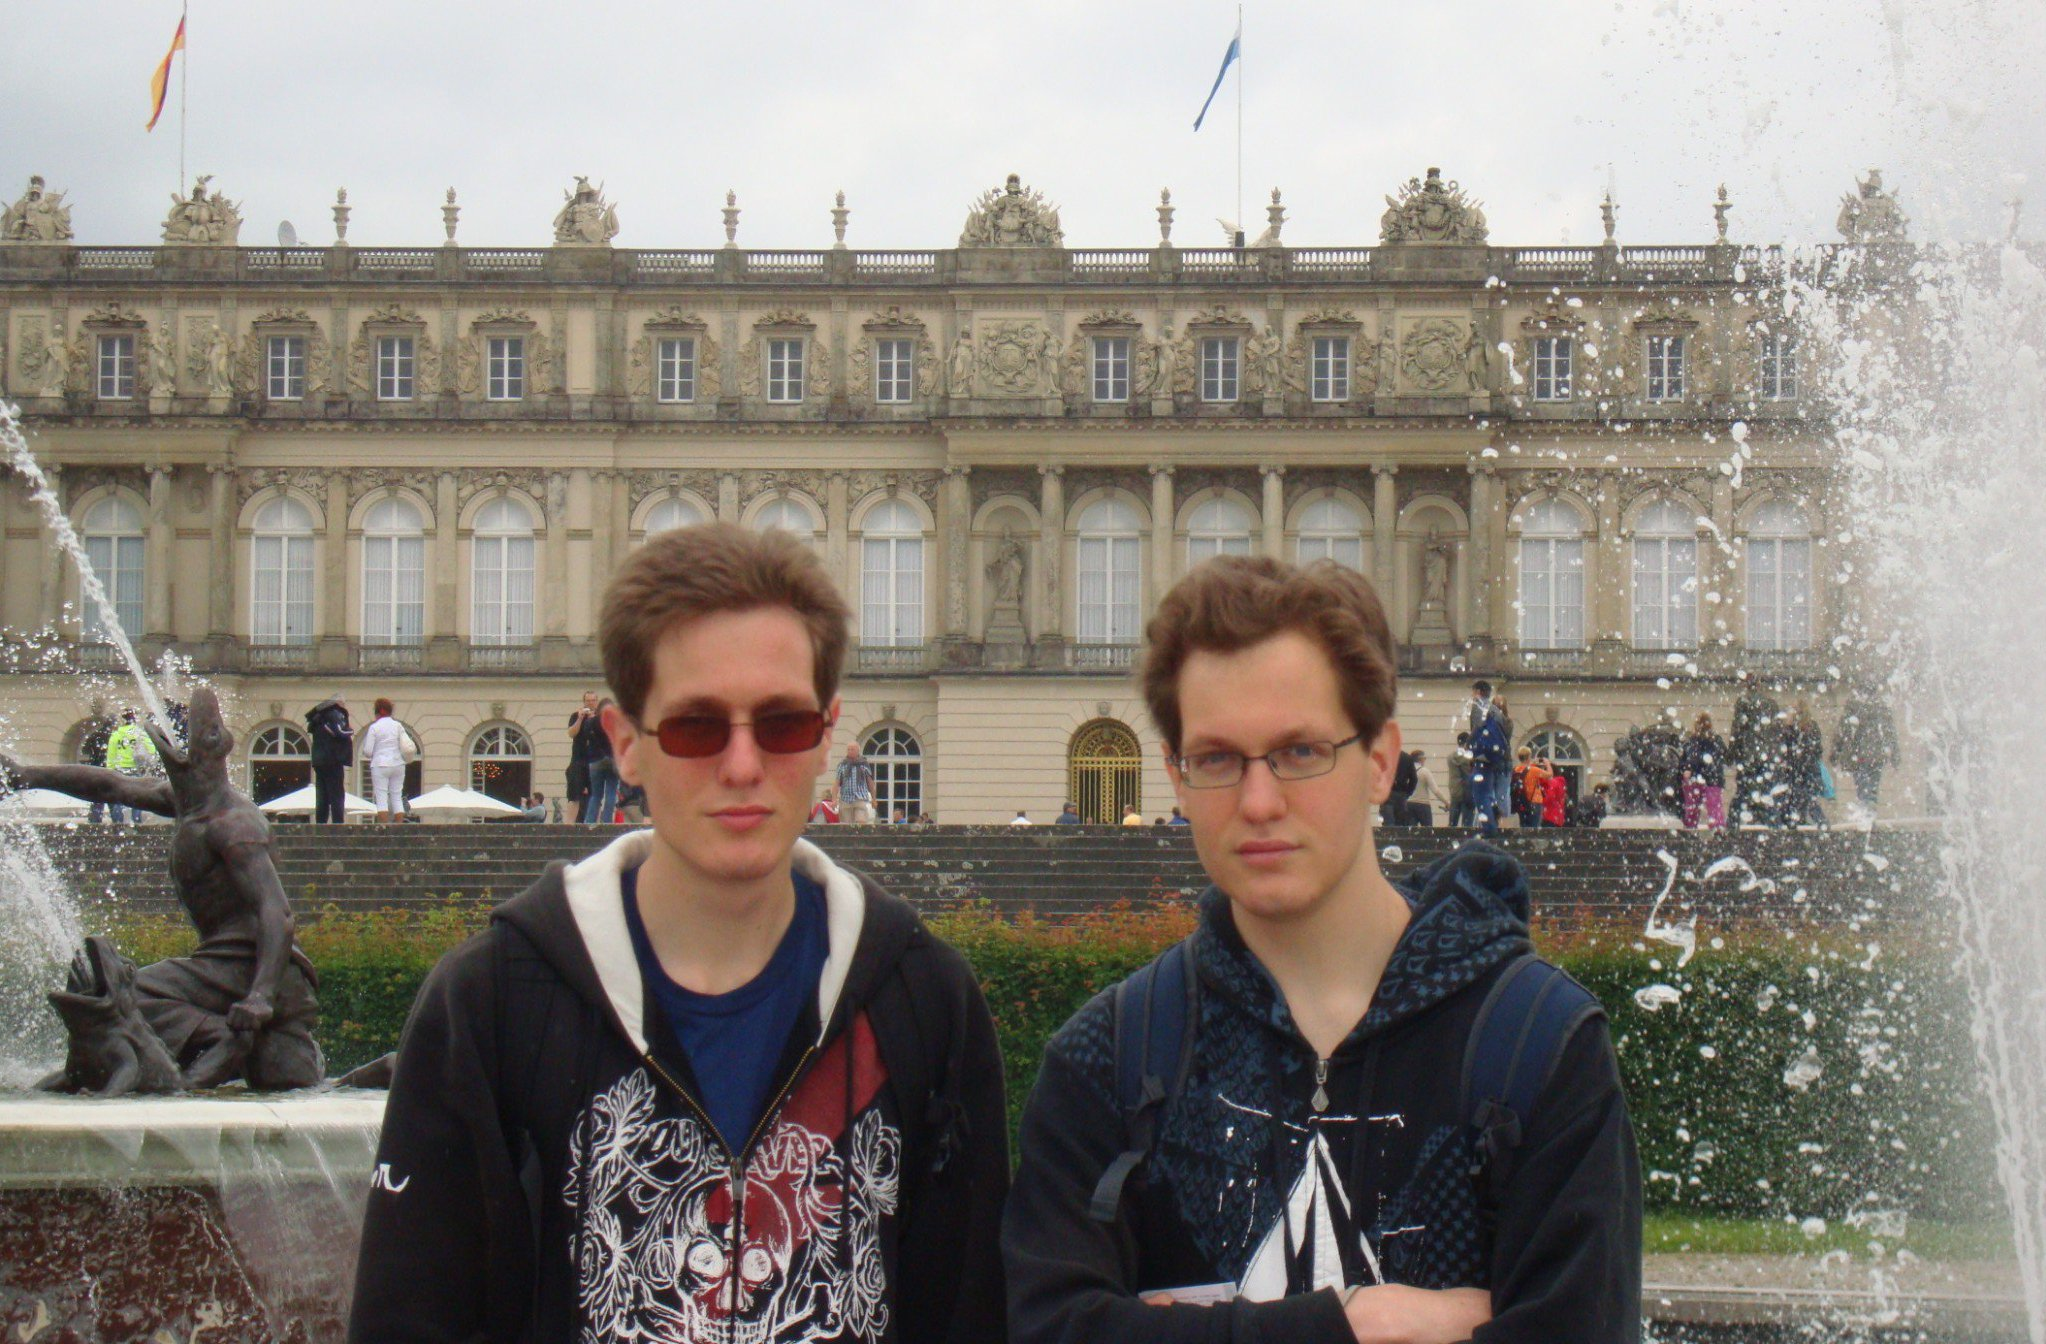
\includegraphics[height=3in]{herrenchiemsee}
\caption{\label{figure2} Myself (left) and my brother Alex (right) at Herrenchiemsee during our two-week stay in Munich.}
\end{figure}
\end{center}

Before starting my internship, the DAAD provided a 2-week language course in Munich which I was able to attend. This was fortunate, since my twin brother was also on the RISE programme (although working far away in Berlin), and so it meant I didn't have to leave England alone. The language course was one of the best parts of my time in Germany, I made good friends with someone on the language course who worked in Munich and we would later visit Ulm and Basel together. Coincidentally, one of the students who was also working near Konstanz happened to be working in Munich for the start of her internship, and so it also gave me a great opportunity to meet someone who I was able to see regularly when working in Konstanz.\\

The language course was excellent, the teachers were friendly and I learnt a good amount of German given it was the first time I'd studied it. The language school also provided a trip to Dachau and the Augustiner Brewery which were both interesting. I also took the opportunity to visit Salzberg and Herrenchiemsee with the other language school students, and the various attractions in Munich such as the Nymphenburger Palace, Hofbrauhaus, Englischer Garten and the art museums. My host family were also very welcoming and were helpful in recommending places to visit in Munich and around Konstanz too.\\

When I first started my internship, my PhD student supervisor explained the basics of the project the research group had been working on and gave me some papers to read to understand the basics. For the first week, I read these papers and watched the other workers going through the standard processes in the small laboratory and clean room. However, after starting work in the clean room independently, I found the work very difficult (due to the handling of strong acids necessary to clean the Silicon samples) and informed my supervisor of my difficulties.\\

\begin{center}
\begin{figure}[htp]
\centering
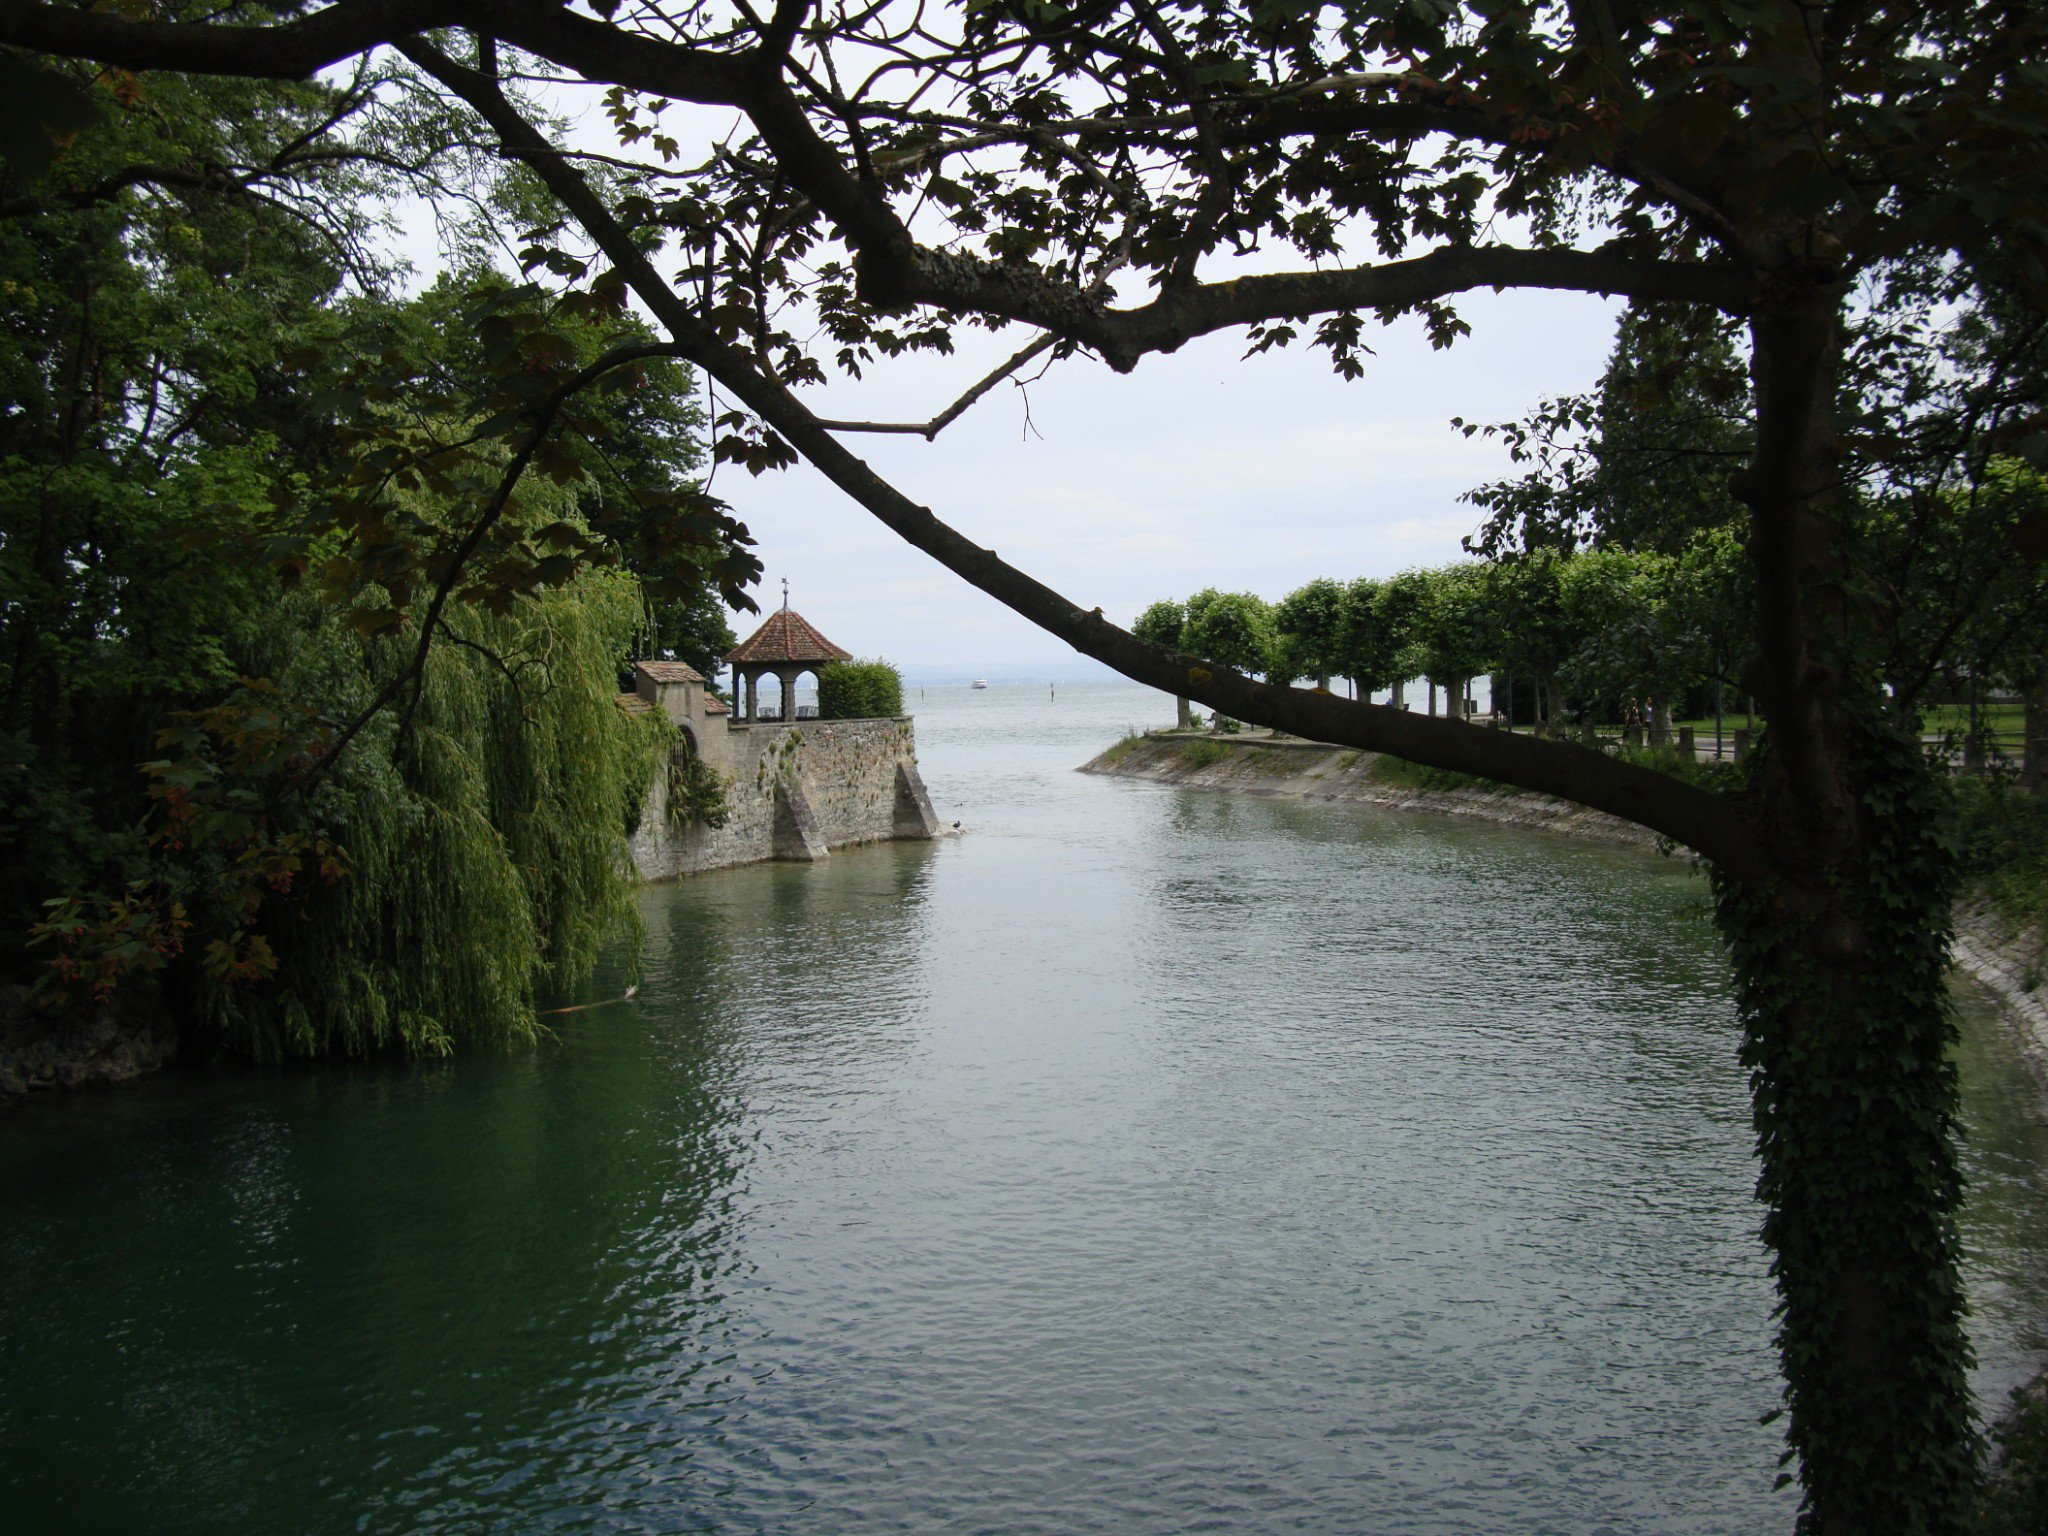
\includegraphics[height=3in]{bodensee}
\caption{\label{figure2} A view of the Bodensee from Konstanz.}
\end{figure}
\end{center}
I then attended the RISE Meeting in Heidelberg. This was excellent, as I had the chance to meet my brother and friends from Munich again, and also to explore Heidelberg. Of particular interest was the Heidelberger Thingst\"{a}tte, an amphitheater constructed during the Nazi era, and the Monastery of St. Michael both at the end of the Philosopher's Walk.\\

After returning from Heidelberg, my supervisor decided it would be better if I worked on the programming for data analysis instead, and I worked on this until the end of my internship, producing my own program that produced spatially resolved plots of the interstitial iron concentration from the measurements of the samples. This was quite interesting work, and I learnt a lot about programming which will certainly be useful in the future. I think this is an important lesson in that if you have any difficulties with your tasks, you should always mention it so others might be able to help.\\

%Heidelberg image
\begin{center}
\begin{figure}[htp]
\centering
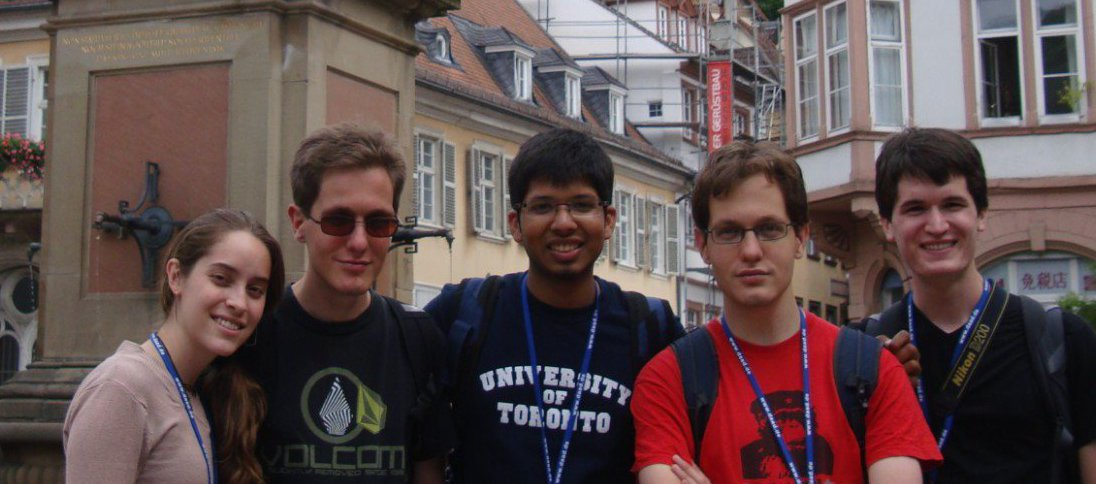
\includegraphics[height=2in]{heidelberg}
\caption{\label{figure2} Myself and other RISE students in Heidelberg.}
\end{figure}
\end{center}
Other highlights of my internship include the day-trip the department made where we canoed along the Bodensee and had a barbecue over an open fire, and hiking around Freiburg with one of the RISE Professional students.\\

Towards the end of the internship it seemed like I wouldn't be able to get the project finished due to some outstanding problems with fitting the data, however I kept trying and fortunately was able to fix all the issues in the penultimate week.\\

Overall I had an excellent time in Germany, and would definitely recommend the RISE programme to any prospective interns. It has made me much more confident in working abroad and travelling independently, and has certainly made me consider working in Germany after graduation.

\end{document}